\documentclass[notitlepage,a4paper,10pt,normalheadings]{article}

% \usepackage{mathpazo} 
\usepackage{ngerman} 
\usepackage[latin1]{inputenc} 
\usepackage[T1]{fontenc} 
\usepackage[pdftex]{graphicx} 
\usepackage[pdftex]{hyperref}

\sloppy

%opening
\title{Anonym Surfen}
\author{Eine Anleitung insbesondere f�r Mozilla Firefox und KDE}
\date{\today}

\hypersetup {
    pdftitle= { Anonym Surfen mit Mozilla Firefox }
    pdfkeywords= {Anonym Surfen Mozilla Firefox Cookies Java-Script Werbung Mixkaskaden Tor Jap }
}


\begin{document}
\maketitle
\tableofcontents

\newpage
\section{Ein Konzept f�r anonymes Surfen}
Das auf den folgenden Seiten vorgestellte Konzept zum spurenarmen Surfen umfasst folgende Punkte:

\begin{enumerate}
\item Die Nutzung datensammelnder Webangebote kann man vermeiden.
\item Die Annahme von Cookies und die Ausf�hrung von JavaScript wird auf vertrauensw�rdige Websites eingeschr�nkt.
\item Werbung, HTML-Wanzen und die Like-Buttons (mit denen Social Networks wie Facebook Daten sammeln) werden durch Filter blockiert.
\item Verr�terische Informationen des Browsers werden entfernt.
\item Risikoreiche und Privacy-unfreundliche Features wie PDF-Reader Plug-Ins, Browser History, Geolocation usw. werden im Browser deaktiviert.
\item HTTPS-Zertifikate werden zus�tzlich validiert, um Man-in-middle Angriffe zu erschweren.
\item Der Datenverkehr kann �ber einen Anonymisierungsdienst geleitet werden. Die verschl�sselte Kommunikation verhindert auch die Auswertung des Internetverkehrs durch mitlesende Dritte wie z.B. unsichere WLAN-Hotspots oder TK�V. (siehe \textit{Anonymymisierungsdienste nutzen})
\end{enumerate}

Mit diesen Ma�nahmen kann es vorkommen, dass Websites nicht wie erwartet funktionieren. Gute Webdesigner verzichteten auf suspekte Technologien, JavaScript wird sinnvoll eingesetzt und der Surfer auf fehlende Freigaben hingewiesen. Cookies sind meist f�r Logins n�tig und Javascript erm�glicht h�bsche Animationen oder Pr�fung von Eingaben.

\begin{center}

\includegraphics[scale=0.75]{../screenshots/cookies_required1.png}
\end{center}

Weniger gute Webseiten liefern seltsame Fehlermeldungen:

\begin{center}
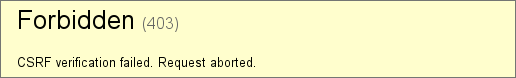
\includegraphics[scale=0.75]{../screenshots/cookies_wrong1.png}
\end{center}

Ganz schlechte Websites machen irgendwas, aber nicht was man erwartet Gelegentlich werden auch Referer oder User-Agent ausgewertet, obwohl es belanglos sein sollte, und Surfer werden nicht auf die notwendigen Freigaben hingeweisen. Hier ist man auf Probieren und Raten angewiesen. Als erstes kann man Cookies freigeben. Wenn das hilft kann man Javascript gezielt f�r einzelne Server freigeben. Ob die Deaktivierung der Schutzma�nahmen die volle Funktionalit�t aufwiegt, muss man bei Bedarf selbst entscheiden.\\

\section{Auswahl des Webbrowsers}
Firefox ist der Webbrowser der Mozilla Foundation. Er ist kostenfrei nutzbar und steht auf der Website des Projektes \footnote{ \href{http://www.mozilla-europe.org/de/firefox}{http://www.mozilla-europe.org/de/firefox}} f�r fast alle Betriebssystem zum Download bereit. Linux-Distributionen enthalten den Browser in der Regel.\\

Debian GNU/Linux enth�lt eine branded version des Browsers unter dem Namen \textit{Iceweasel}, allerding oft in einer veralteten Version. Das Mozilla Debian Team stellt eine aktuelle Version in einem extra Repository \footnote{ \href{http://mozilla.debian.net}{http://mozilla.debian.net}} bereit.\\

Firefox kann durch viele von der Community entwickelte Add-ons und Anpassungen in der Konfiguration zu einem sicheren und privacy-freundlichen Browser aufgewertet werden. Ich beschr�nke mich im folgenden auf diesen einen Browser. Das ist schon sehr umfangreich, wenn man es gut machen will.

\subsubsection*{JonDoFox}
Der JonDoFox\footnote{ \href{https://www.anonym-surfen.de/jondofox.html}{https://www.anonym-surfen.de/jondofox.html}} ist ein Browser-Profil f�r Firefox, dass alle Einstellungen umsetzt, die auf den folgenden Seiten beschrieben werden. Nach der Installation von Mozilla Firefox ist das JonDoFox-Profil zus�tzlich zu installieren - fertig. Zuk�nftig fragt Firefox bei jedem Start, welches Profil genutzt werden soll. JonDoFox ist f�r anonymes Surfen mit JonDonym entwickelt worden, kann aber auch ohne Anonymisierungsdienst verwendet werden, indem man in der Statuszeile unten rechts auf \textit{Kein Proxy} oder \textit{Benutzerdefiniert} umschaltet.

\begin{center}
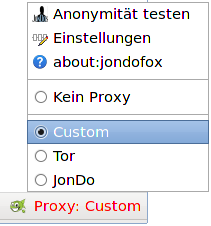
\includegraphics[scale=0.75]{../screenshots/jondofox-proxy-ohne.png}
\end{center}

Wenn man den Proxy \textit{Benutzerdefiniert} w�hlt, kann die User-Agent Kennung modifiziert werden. Das ist vor allem f�r Nutzer seltener Betriebssysteme sinnvoll, um sich in der Masse der Windows-Nutzer zu verstecken. In den Einstellungen des JonDoFox kann man f�r Benutzerdefinierte Proxys den \textit{Firefox 17.0 f�r Windows} (JonDo) oder \textit{Firefox 10.0 f�r Windows} (Tor) als Fake zu nutzen. Mit dieser kleinen Anpassung erh�lt man einen optimal konfigurierten Browser. Das folgende Kapitel kann man trotzdem lesen oder �berfliegen, um die damit verbundenen Einschr�nkungen besser zu verstehen.\\

\begin{figure}[htb]
\begin{center}
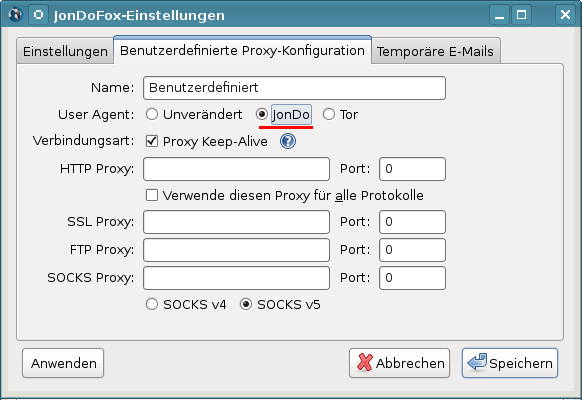
\includegraphics[scale=0.7]{../screenshots/jondofox-ua-ohne.png}
\caption{User-Agent Kennung konfigurieren}
\label{abb:jondofox-ua}
\end{center}
\end{figure}

Eine kurze Einf�hrung in den Umgang mit JonDoFox gibt es im Kapitel Anonymisierungsdienste.

\subsubsection*{JoDoBrowser}
Der JonDoBrowser\footnote{ \href{https://www.anonym-surfen.de/jondobrowser.html}{https://www.anonym-surfen.de/jondobrowser.html}} ist nicht nur sicher konfiguriert sondern enth�lt auch Modifikationen im Source Code von Mozilla Firefox, um eine h�here Anonymit�t zu bieten. Die aktuelle Beta Version arbeitet stabil und kann meiner Meinung nach f�r die t�gliche Arbeit eingesetzt werden.\\

Standardm��ig ist die Proxy-Umschaltung im JonDoBrowser deaktiviert. Das erweiterte Men� muss erst in den Einstellungen des JonDoFox-XPI (siehe Bild \ref{abb:proxyfreigeben}) aktiviert werden. Dann kann man wie beim JonDoFox auf \textit{``Kein Proxy``} umschalten und ohne Anonymisierungsdienst spurenarm surfen.

\begin{figure}[htb]
\begin{center}
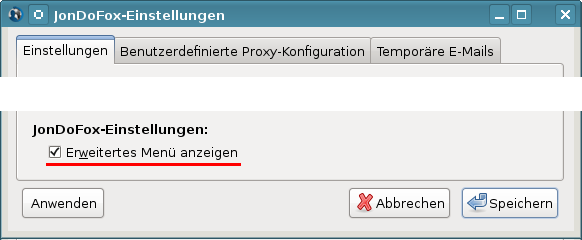
\includegraphics[scale=0.7]{../screenshots/jondobrowser-proxy-aktivieren.png}
\caption{Proxy-Umschaltung im JonDoBrowser freigeben}
\label{abb:proxyfreigeben}
\end{center}
\end{figure}
\section{Cookies}
Cookies werden f�r die Identifizierung des Surfers genutzt. Neben der erw�nschten Identifizierung um personalisierte Inhalte zu nutzen, beispielsweise einen Web-Mail-Account oder um Eink�ufe abzuwickeln, werden sie auch f�r das Tracking von Nutzern verwendet.\\

Der Screenshot Bild \ref{abb:cookiespiegel} zeigt die Liste der Cookies, die bei einem einmaligen Aufruf der Seite \textit{www.spiegel.de} gesetzt wurden. Neben den Cookies von \textit{spiegel.de} zur Z�hlung der Leser setzen gleich mehrere datensammelnde Werbeserver Cookies und au�erdem Z�hldienste (quality-chanel.de, ivwbox.de), welche die Reichweiten von Online-Publikationen auswerten.\\

\begin{figure}[p]
\begin{center}
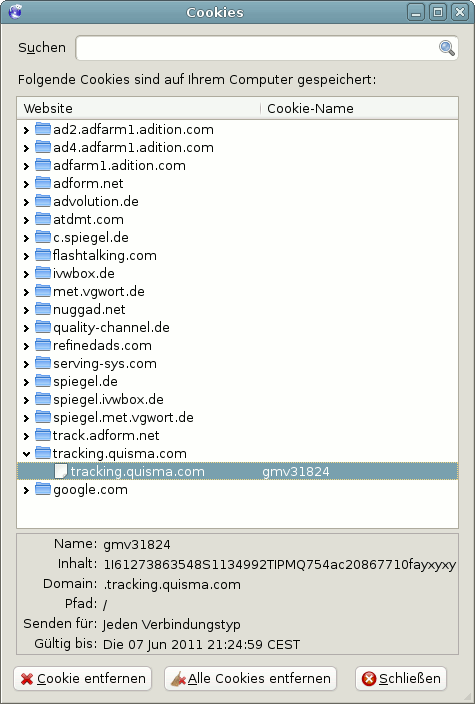
\includegraphics[scale=0.75]{../screenshots/cookies_spiegel.png}
\caption{Liste der Cookies beim Besuch von Spiegel-Online}
\label{abb:cookiespiegel}
\end{center}
\end{figure}

Es ist nicht ungew�hnlich, dass popul�re Webseiten mehrere Datensammler einbinden. Eine Studie der Universit�t Berkeley \footnote{ \href{http://heise.de/-1288914}{http://heise.de/-1288914}}  hat 2011 beim Surfen auf den TOP100 Webseiten 5.675 Cookies gefunden (ohne Login oder Bestellung). 4.914 Cookies wurden von Dritten gesetzt, also nicht von der aufgerufenen Webseite. Die Daten wurden an mehr als 600 Server �bermittelt. Spitzenreiter unter den Datensammlern ist Google, 97\% der popul�ren Webseiten setzen Google-Cookies.\\

Sinnvoll ist ein \textbf{Whitelisting} f�r die Behandlung von Cookies:

\begin{enumerate}
\item Standardm��ig wird die Annahme von Cookies verweigert.
\item F�r vertrauensw�rdige Websites, welche die Nutzung von Cookies zur Erreichung der vollen Funktion ben�tigen, werden Ausnahmen zugelassen.
\item Die f�r den Zugriff auf personalisierte Inhalte gespeicherten Cookies sollten beim Schlie�en des Browsers automatisch gel�scht werden. Einige Websites verwenden diese Cookies auch nach dem Logout f�r das User-Tracking.
\end{enumerate} 

Fast alle Login-Seiten, welche Cookies zur Identifizierung des Surfers verwenden, weisen mit einem kleinen Satz auf die notwendigen Freigaben hin. Treten beim Login seltsame Fehler auf, z.B. st�ndig die Fehlermeldung \textit{FALSCHES PASSWORT}, verweigert der Browser wahrscheinlich die Annahme von Cookies. Die Website sollte in die Liste der vertrauensw�rdigen Websites aufgenommen werden.\\



\section{JavaScript}
JavaScript ist eine der Kerntechniken des modernen Internet, birgt aber auch einige Sicherheitsrisiken.
\begin{enumerate}
\item Mit Hilfe von Javascript kann man ein Vielzahl von Informationen �ber den Browser und das Betriebssystem auslesen. Bildschirmgr��e, Farbeinstellungen, installierte Plugins und Hilfs-Applikationen.... Die Website \href{http://browserspy.dk}{http://browserspy.dk} zeigt eine umfangreiche Liste.\\

Diese Informationen k�nnen zu einem individuellen Fingerabdruck verrechnet werden. Anhand dieses Fingerabdruck kann der Surfer wiedererkannt werden, auch wenn er die IP-Adresse mit VPNs oder Anonymisierungsdiensten verschleiert. Die EFF geht davon aus, dass diese Methode von vielen Datensammlern genutzt wird.
\begin{itemize}
 \item \textit{Yahoo! Web Analytics} nutzt Javascript Tracking Code, wenn Cookies blockiert werden.
 \begin{quote}
  \textit{In case Yahoo! Web Analytics cannot set a cookie, the system can still retrieve information from the JavaScript tracking code, the IP address and the web browser user agent. \footnote{ \href{http://help.yahoo.com/l/us/yahoo/ywa/documentation/install\_guide/ig\_get\_started.html}{http://help.yahoo.com/l/us/yahoo/ywa/documentation/install\_guide/ig\_get\_started.html}} }
 \end{quote}  
 \item Ein weiteres Beispiel ist die Firma \textit{bluecave} \footnote{ \href{http://www.bluecava.com}{http://www.bluecava.com}}. Das Trackingscript \textit{BCAL5.js} sammelt Informationen zur verwendeten Software, installierte Schriftarten, Bildschirmgr��e, Browser Plug-ins und ein paar mehr Daten, um daraus einen individuellen Fingerprint zu berechnen. \textit{bluecave} protzt damit, 99\% der Surfer zu erkennen.
 \item Der Trackingdienst Multicounter \footnote{ \href{http://www.multicounter.de/features.html}{http://www.multicounter.de/features.html}} und die Google Suche speichern die per Javascript ausgelesene Bild�schirm�gr��e als individuelles Merkmal.
\end{itemize}

\item Einige EverCookie Techniken nutzen Javascript, um zus�tzliche Markierungen im Browser zu hinterlegen und gel�schte Tracking Cookies wiederherzustellen.

\item Durch Einschleusen von Schadcode k�nnen Sicherheitsl�cken ausgenutzt und der der Rechner kann kompromittiert werden. Das Einschleusen von Schadcode erfolgt dabei auch �ber vertrauensw�rdige Webseiten, beispielsweise mit Cross Site Scripting, wenn diese Websites nachl�ssig programmiert wurden. Werbebanner k�nnen ebenfalls b�s�artigen Javascriptcode transportieren. Im Januar 2013 lieferten die Server des Werbe�netzwerkes OpenX Scripte aus, die Rechner durch Ausnutzung mehrerer Sicherheitsl�cken im Internet Explorer kompromittierten.\footnote{ \href{http://heise.de/-1787511}{http://heise.de/-1787511}}
\end{enumerate}

Ein generelles Abschalten ist heutzutage nicht sinnvoll. �hnlich dem Cookie-Management ben�tigt man ein Whitelisting, welches JavaScript f�r vertrauensw�rdige Websites zur Erreichung der vollen Funktionalit�t erlaubt, im allgemeinen jedoch deaktiviert. Gute Webdesigner weisen den Nutzer darauf hin, dass ohne Javascript eine deutliche Einschr�nkung der Funktionalit�t zu erwarten ist. 



\section{Werbung, HTML-Wanzen und Social Media}
Die auf vielen Websites eingeblendete \textbf{Werbung }wird von wenigen Servern bereitgestellt. Diese nutzen h�ufig (eigentlich immer) die damit gegebenen M�glichkeiten, das Surfverhalten �ber viele Websites hinweg zu erfassen. Mit Hilfe von listen- und musterbasiert Filtern kann der Zugriff auf Werbung sowie die von diesen Servern genutzten Cookies unterbunden werden.\\

Hinweis: Viele Angebote im Web werden �ber Werbung finanziert, da die Nutzer meist nicht bereit sind, f�r diese Angebote zu bezahlen. Die Redaktion von Heise.de hat ein kurzes Statement\footnote{ \href{http://www.heise.de/Adblocker-auf-heise-online-1164703.html}{http://www.heise.de/Adblocker-auf-heise-online-1164703.html}} zu Werbung auf Heise online ver�ffentlicht und erkl�rt, wie sie einzelne Webangebote durch Freigaben im Werbeblocker unterst�tzen k�nnen.\\

Bei \textbf{HTML-Wanzen} (sogenannten Webbugs) handelt es sich um 1x1-Pixel gro�e transparente Bildchen, welche in den HTML-Code einer Webseite oder einer E-Mail eingebettet werden. Sie sind f�r den Nutzer unsichtbar und werden beim Betrachten einer Webseite oder beim �ffnen der E-Mail von einem externen Server geladen und erm�glichen es dem Betreiber des Servers, das Surfverhalten website�bergreifend zu verfolgen.\\

Hinweis: das System METIS\footnote{ \href{http://www.vgwort.de/metis.php}{http://www.vgwort.de/metis.php}} der VG Wort verwendet HTML-Wanzen, um die Besucher von Online-Angeboten zu z�hlen und anhand der Ergebnisse Tantiemen an Autoren auszuzahlen.\\

Facebook und andere Sociale Netze verwenden sogenannte \textbf{Like Buttons}, um Daten zu sammeln. Die Verwendung der Like Buttons ist nach Ansicht von Thilo Weichert (ULD) nicht mit deutschen Datenschutzrecht vereinbar. Deutsche Webseitenbetreiber sind aufgefordert, die Facebook Buttons von ihren Seiten zu entfernen\footnote{ \href{https://www.datenschutzzentrum.de/facebook/}{https://www.datenschutzzentrum.de/facebook}}. Mit dem Aufruf einer Webseite, die den Like Button enth�lt, werden Daten an Facebook �bertragen und dort ausgewertet.\\

Forscher der Universit�t Cambridge (Gro�britannien) konnten im Rahmen einer Untersuchung durch Auswertung der Klicks auf Facebook Like Buttons die sexuelle Orientierung und politische Einstellung der Teilnehmer vorhersagen\footnote{ \href{http://heise.de/-1820638}{http://heise.de/-1820638}}. Man verr�t mit einem Klick auf einen Like Button m�glicherweise Informationen, die man nicht im Netz ver�ffentlichen m�chte. 

\subsection{Tracking-Filter f�r Firefox}
Es gibt mehrere Add-ons f�r Firefox, die Werbung und Trackingelemente blockieren. Das Center for Internet and Society der Stanford Law School hat in einer Analyse vom September 2011 einige L�sungen verglichen \footnote{ \href{https://cyberlaw.stanford.edu/node/6730}{https://cyberlaw.stanford.edu/node/6730}}. Die Ergebnisse in Bild \ref{abb:trackingfilter} zeigen: keine L�sung ist perfekt.\\

\begin{figure}[htb]
\begin{center}
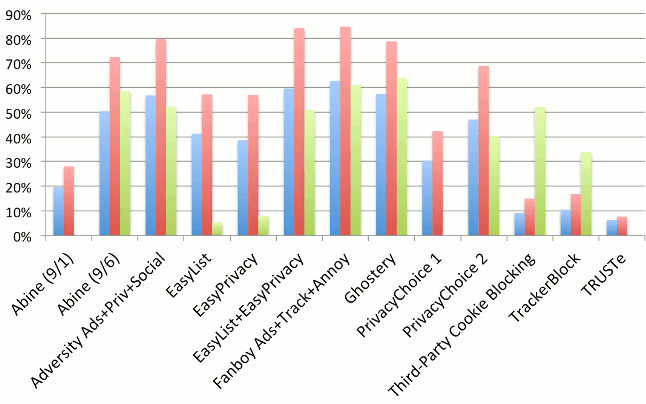
\includegraphics[scale=1.0]{../screenshots/tracking-blocker.png}
\caption{Effektivit�t verschiedener Tracking-Filter}
\label{abb:trackingfilter}
\end{center}
\end{figure}

Aufgrund der Flexibilit�t bei der Einbindung verschiedener Filterlisten empfehle ich \textit{AdBlock Plus}. Mit den Easylist Filterlisten erreichten das Add-on bei dem Test mit die besten Ergebnisse. Die Listen werden st�ndig weiterentwickelt. Es gibt als Zusatz eine spezielle Filterliste f�r deutsche Webseiten.\\

Zus�tzlich zur den Blocklisten\textit{ EasyList+Germany} und \textit{EasyPrivacy} sollte man noch eine Liste abonnieren, die die Social Media Buttons blockiert, z.B. \textit{SocialMediaBlock} von MontzA.\\

\textit{FanBoy} arbeitet seit 2010 mit EasyList zusammen, daher die �hnlich guten Ergebnisse. \textit{Ghostery} schneidet im Test auch gut ab und wird oft empfohlen. Es gibt aber immer wieder Probleme mit Ghostery auf einigen Webseiten, da das Add-on kein Whitelisting kennt. Au�erdem arbeitet es mit einer festen Blockliste, die nicht flexibel erweitert oder kombiniert werden kann. 
\section{HTTP-Header filtern}
Neben der Verwendung von Cookies wird auch der Inhalt des HTTP-Header f�r die Gewinnung von Informationen �ber den Surfer genutzt. Das Projekt \textit{Panopticlick} \footnote{ \href{http://panopticlick.eff.org/}{http://panopticlick.eff.org}} der EFF.org zeigt, dass anhand des Fingerprint des HTTP-Headers 80\% der Surfer eindeutig erkennbar sind. Eine Verkn�pfung dieser Information �ber mehrere Websites hinweg kann eine Verfolgung von Nutzern erm�glichen. Kombiniert man diese Verfolgung mit Daten von Sozialen Netzen (Facebook, Xing), ist eine vollst�ndige Deanonymiserung m�glich.
\begin{itemize}
\item Beispiel \textbf{User-Agent}: Die meisten Browser senden Informationen �ber den verwendeten Browser und das Betriebssystem. Ein Beispiel zeigt, wie detailliert der Browser Auskunft gibt:
\begin{verbatim}
Mozilla/5.0 (Macintosh; U; PPC Mac OS X; de-DE) AppleWebKit/419.3 
(KHTML, like Gecko) Safari/419.3
\end{verbatim}
Beim US-Reiseportal Orbitz werden Surfern mit MacOS (am User-Agent erkennbar) die Hotelzimmer 20-30 Dollar teuerer angeboten, als anderen Kundern\footnote{ \href{http://heise.de/-1626368}{http://heise.de/-1626368}}. Au�erdem k�nnen anhand der Informationen gezielt L�cken in der verwendeten Software ausgenutzt werden.\\


\item Erg�nzende Informationen wie zum Beispiel die bevorzugte \textbf{Sprache}, installierte \textbf{Schrift�arten} und \textbf{Gr��e des Browserfensters} k�nnen einen individuellen Fingerprint des Browsers ergeben. Viele Werte k�nnen per Javascript ausgelesen werden Bei der Google-Suche und beim Trackingdienst Multicounter\footnote{ \href{http://www.multicounter.de/features.html}{http://www.multicounter.de/features.html}} wird die innere Gr��e des Browser�fensters ausgelesen. Die Firma bluecave\footnote{ \href{http://www.bluecava.com/}{http://www.bluecava.com}} nutzt z.B. im Trackingscript \textit{BCAL5.js} u.a. Informationen �ber installierte Schriftarten.\\

Deshalb sollte man Javascript nur f�r vertrauensw�rdige Webseiten erlauben und das Auslesen der Werte behindern (soweit m�glich).
\end{itemize} 


\input{surfen_filter_privoxy}
\input{surfen_filter_proxomitron}
\newpage
\subsection{Mozilla Firefox konfigurieren}
Auch Mozilla Firefox kann einen installierten Content-Filter nutzen.\\

\begin{figure}[htb]
\begin{center}
\includegraphics[scale=0.60]{../screenshots/browser_20.png}
\caption{Einstellungsdialog in Firefox 2.0}
\label{abb:firefox_einst_verb_20}
\end{center}
\end{figure}

Im Browser \textbf{Firefox 1.5} ist hierf�r der Dialog \textit{Einstellungen} zu �ffnen und zur Sektion \textit{Allgemein} zu wechseln. Die Konfiguration des genutzten Proxy erreicht man �ber den Button \textit{Verbindungs-Einstellungen}.\\

Im Browser \textbf{Firefox 2.0} ist der Dialog \textit{Einstellungen} �berarbeitet worden. Die Verbindung zum Internet kann in der Sektion \textit{Erweitert} auf dem Reiter \textit{Netzwerk} konfiguriert werden. Hier findet man den Button \textit{Einstellungen}, der ebenfalls den in Bild \ref{abb:firefox_einst_verb} gezeigte Dialog �ffnet.\\

\begin{figure}[htb]
\begin{center}
\includegraphics[scale=0.60]{../screenshots/browser_2.png}
\caption{Verbindungs-Einstellungen}
\label{abb:firefox_einst_verb}
\end{center}
\end{figure}

Es ist die Option \textit{manuelle Proxy-Konfiguration} zu aktivieren, als Host der eigene Rechner mit \textit{localhost} anzugeben und der Port einzutragen, an welchem der Content-Filter lauscht. F�r Proxomitron ist Port \textit{8080} anzugeben, f�r Privoxy Port \textit{8118}.\\

Au�erdem kann eine Liste von Ausnahmen angegeben werden, eine Liste von Websites, welche ohne Content-Filter besucht werden sollen. Hier sind alle vertrauensw�rdigen Websites einzutragen, welchen mit eingeschaltetem Content-Filter nicht korrekt funktionieren. In jedem Fall sollten lokale Webseiten nicht gefiltert werden (\textit{localhost, 127.0.0.1}).\\

L�uft der Content-Filter nicht auf dem eigenen Rechner sondern auf einem Gateway, ist statt \textit{localhost} der Name oder die IP-Adresse dieses Rechners einzutragen.
 
Anonymisierungsdienste verwischen die Spuren im Internet bei der Nutzung herk�mmlicher Webdienste. Die verschl�sselte Kommunikation verhindert auch ein Belauschen des Daten�verkehrs durch mitlesende Dritte. Diese Dienste sind f�r den anonymen Zugriff auf Websites geeignet und erm�glichen auch unbeobachtete, private Kommunikation via E-Mail, Jabber, IRC...\\

Die unbeobachtete, private Kommunikation schafft keine rechtsfreien R�ume im Internet, wie Demagogen des �berwachungsstaates immer wieder behaupten. Sie ist ein grundlegendes Menschenrecht, das uns zusteht. Nach den Erfahrungen mit der Diktatur Mitte des letzten Jahrhunderts findet man dieses Grundrecht in allen �bergeordneten Normenkatalogen, von der UN-Charta der Menschenrechte bis zum Grundgesetz.\\

Anonymisierungsdienste sind ein Hammer unter den Tools zur Verteidigung der Privatsph�re, aber nicht jedes Problem ist ein Nagel. Das Tracking von Anbietern wie DoubleClick verhindert man effektiver, indem man den Zugriff auf Werbung unterbindet. Anbieter wie z.B. Google erfordern es, Cookies und JavaScript im Browser zu kontrollieren. Anderenfalls wird man trotz Nutzung von Anonymisierungsdiensten identifiziert.

\section{Warum sollte man diese Dienste nutzen?}
Anonymisierungsdienste verstecken die IP-Adresse des Nutzers und verschl�sseln die Kommunikation zwischen Nutzer und den Servern des Dienstes. Au�erdem werden spezifischer Merkmale modifiziert, die den Nutzer identifizieren k�nnten (Browser-Typ, Betriebssystem....).
\begin{enumerate}
 \item \textbf{Profilbildung:} Nahezu alle gro�en Suchmaschinen generieren Profile von Nutzern, Facebook u.a. Anbieter speichern die IP-Adressen f�r Auswertungen. Nutzt man Anonymisierungsdienste, ist es nicht m�glich, diese Information sinnvoll auszuwerten.
 \item \textbf{Standortbestimmung:} Die Anbietern von Webdiensten k�nnen den Standort des Nutzers nicht via Geolocation bestimmen. Damit ist es nicht m�glich:
\begin{itemize}
 \item die Firma identifizieren, wenn der Nutzer in einem Firmennetz sitzt.
 \item bei mobiler Nutzung des Internet Bewegungsprofile zu erstellen.
\end{itemize}
\item \textbf{Belauschen durch Dritte:} Die verschl�sselte der Kommunikation mit den Servern des Anonymisierungsdienstes verhindert ein Mitlesen des Datenverkehrs durch Dritte in unsicheren Netzen. (Internet Cafes, WLANs am Flughafen oder im Hotel, TK�V...)
\item \textbf{Rastern:} Obwohl IP-Adressen die Identifizierung von Nutzern erm�glichen, sind sie rechtlich in vielen L�ndern ungen�gend gesch�tzt. In den USA k�nnen sie ohne richterliche Pr�fung abgefragt werden. Die TK-Anbieter genie�en Straffreiheit, wenn sie die nicht vorhandenen Grenzen �bertreten. Wenig verwunderlich, dass man IP-Adressen zur t�glichen Rasterfahndung nutzt. Facebook gibt t�glich 10-20 IP-Adressen an US-Beh�rden, AOL �bergibt 1000 Adressen pro Monat\dots
\item \textbf{Vorratsdatenspeicherung:} Ein Schreiben des Bundesdatenschutzbeauftragen an das Bundesverfassungsgericht macht viele unglaubliche Verst��e gegen die Nutzung der VDS-Daten offenkundig. Es werden h�ufig mehr Daten gespeichert, als gesetzlich vorgegeben. Auch die Bedarfstr�ger halten sich nicht an die Vorgaben des BVerfG.
\begin{quote}
   Zitat: \textit{So haben mir s�mtliche Anbieter mitgeteilt, dass es recht h�ufig vorkomme, dass Beschl�sse nicht den formellen Anforderungen \dots gen�gen. Wenn die Anbieter in derartigen F�llen entsprechenden Auskunftsersuchen nicht nachk�men, w�rde ihnen oft die Beschlagnahme von Servern oder die Vernehmung der leitenden Angestellten als Zeugen angedroht, um auf diesem Wege eine Auskunft zu erzwingen.}
\end{quote}
Die Telekom hat in zwei Monaten 2198 Anfragen beantwortet und dabei wahrscheinlich zu 70\% auf VDS-Daten zur�ck gegriffen. Auch nachdem die Vorratsdatenspeicherung offiziell vom BVerfG beendet wurde, speichern alle Telekommunikationsanbieter weiterhin VDS-�hnliche Datenberge �ber mehrere Wochen.
\item \textbf{Zensur:} Der Datenverkehr kann vom Provider oder einer restriktiven Firewall nicht manipuliert oder blockiert werden. Anonymisierungsdienste erm�glichen einen unzensierten Zugang zum Internet. Sie k�nnen sowohl die ``Great Firewall'' von China und Mauretanien durchtunneln sowie die in westeurop�ischen L�ndern verbreitet Zensur durch Kompromittierung des DNS-Systems.
\item \textbf{Repressionen:} Blogger k�nnen Anonymisierungsdienste nutzen, um kritische Informationen aus ihrem Land zu verbreiten ohne die Gefahr pers�nlicher Repressionen zu riskieren. F�r Blogger aus S�dafrika, Syrien oder Burma ist es teilweise lebenswichtig, anonym zu bleiben. Iran wertet Twitter-Accounts aus, um Dissidenden zu beobachten
\item \textbf{Leimruten:} Einige Websites werden immer wieder als Honeypot genutzt. Ein Beispiel sind die Leimrute des BKA. In mehr als 150 F�llen wurden die Fahndungseiten von LKAs oder des BKA als Honeypot genutzt und die Besucher der Webseiten in Ermittlungen einbezogen \footnote{ \href{http://heise.de/-1704448}{http://heise.de/-1704448}}. Surfer wurden identifiziert und machten sich verd�chtig, wenn sie sich auff�llig f�r bestimmte Themen interessieren.
\item \textbf{Geheimdienste:} Sicherheitsbeh�rden und Geheimdienste k�nnen mit diesen Diensten ihre Spuren verwischen. Nicht immer geht es dabei um aktuelle Operationen. Die Ver�ffentlichung der IP-Adressbereiche des BND bei Wikileaks erm�glichte interessante Schlussfolgerungen zur Arbeitsweise des Dienstes. Beispielsweise wurde damit bekannt, dass der BND gelegentlich einen bestimmten Escort Service in Berlin in Anspruch nimmt.
\item \textbf{Belauschen durch den Dienst:} Im Gegensatz zu einfachen VPNs oder Web-Proxys sch�tzen die hier vorgestellten Anonymisierungsienste auch gegen Beobachtung durch die Betreiber des Dienstes selbst. Die mehrfache Verschl�sselung des Datenverkehrs und die Nutzung einer Kette von Servern verhindert, dass einzelne Betreiber des Dienstes die genutzten Webdienste einem Nutzer zuordnen k�nnen.
\end{enumerate}

\section{Tor Onion Router und JonDonym}
Ein kurzer, oberfl�chlicher Vergleich soll die technischen Unterschiede zwischen verschiedenen Diensten zeigen und Hilfe bei der Entscheidung bieten.

\subsubsection*{Tor Onion Router}
Tor nutzt ein weltweit verteiltes Netz von 2400 aktiven Nodes. Aus diesem Pool werden jeweils 3 Nodes f�r eine Route ausgew�hlt. Die Route wechselt regelm��ig in kurzen Zeitabst�nden. Die zwiebelartige Verschl�sselung sichert die Anonymit�t der Kommunikation. Selbst wenn zwei Nodes einer Route kompromittiert wurden, ist eine Beobachtung durch mitlesende Dritte nicht m�glich.\\

\begin{figure}[htb]
\begin{center}
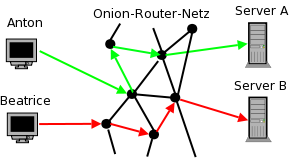
\includegraphics[scale=0.55]{../grafiken/tor.png}
\caption{Prinzip von Tor}
\label{abb:tor_prinzip}
\end{center}
\end{figure}

Da die Route st�ndig wechselt, m�sste ein gro�er Teil des Netztes kompromittiert worden sein, um einen Zusammenhang von Surfer und angefragter Webseite herstellen zu k�nnen.\\

Die weltweite Verteilung der Nodes und der hohe Anteil privater Rechner mit langsamer Internetanbindung kann zu deutlich langsameren Downloads f�hren.\\

Tor ist neben Surfen auch f�r IRC, Instant-Messaging, den Abruf von Mailboxen oder Anderes nutzbar. Dabei versteckt Tor nur die IP-Adresse! F�r die sichere �bertragung der Daten ist SSL- oder TLS-Verschl�sselung zu nutzen. Sonst besteht die M�glichkeit, dass sogenannte \textit{Bad Exit Nodes} die Daten belauschen und an Userkennungen und Passw�rter gelangen.\\

Der Inhalt der Kommunikation wird 1:1 �bergeben. F�r anonymes Surfen bedarf es weiterer Ma�nahmen, um die Identifizierung anhand von Cookies, der HTTP-Header, ETags aus dem Cache oder Javascript zu verhindern. Mozilla Firefox wird mit TorButton oder JonDoFox optimal eingestellt.\\

Verschiedene Sicherheitsforscher demonstrierten, dass es mit schn�ffelnden \textit{Bad Exit Nodes} relativ einfach m�glich ist, Daten der Nutzer zu sammeln. 
\begin{itemize}
 \item Dan Egerstad demonstrierte, wie man in kurzer Zeit die Account Daten von mehr als 1000 E-Mail Postf�chern erschn�ffeln kann, u.a. von 200 Botschaften.
\item Auf der Black Hack 2009 wurde ein Angriff auf die HTTPS-Verschl�sselung beschrieben. In Webseiten wurden HTTPS-Links durch HTTP-Links ersetzt. Innerhalb von 24h konnten mit einen Tor Exit Node folgende Accounts erschn�ffelt werden: 114x Yahoo, 50x GMail, 9x Paypal, 9x Linkedin, 3x Facebook. Im Februar 2012 haben mehrere russische Extis-Nodes diesen Angriff praktisch umgesetzt.
\item Die Forscher um C. Castelluccia nutzten f�r ihren Aufsatz \textit{Private Information Disclosure from Web Searches (The case of Google Web History)} einen schn�ffelnden Tor Exit Node, um private Informationen von Google Nutzern zu gewinnen.
\item Um reale Zahlen f�r das Paper \textit{Exploiting P2P Applications to Trace and Profile Tor Users} zu generieren, wurden 6 modifizierte Tor Nodes genutzt und innerhalb von 23 Tagen mehr als 10.000 User deanonymisiert.
\end{itemize}

Man kann davon auszugehen, dass die Geheimdienste verschiedener L�nder ebenfalls im Tor-Netz aktiv sind und sollte die Hinweise zur Sicherheit beachten: sensible Daten nur �ber SSL-verschl�sselte Verbindungen �bertragen, SSL-Warnungen nicht einfach wegklicken, Cookies und Javascript deaktivieren\dots Dann ist Tor f�r anonyme Kommunikation geeignet.\\

Tor bietet nicht nur anonymen Zugriff auf verschiedene Services im Web. Die Tor Hidden Services bieten M�glichkeiten, anonym und zensurresistent zu publizieren.

\subsubsection*{JonDonym} 
JonDonym arbeitet mit wenigen festen Mix-Kaskaden, bestehend aus zwei oder drei Knoten. Diese Knoten sind leistungsf�hige Computer mit schneller Internetanbindung. Die Daten der einzelnen Nutzer werden mehrfach verschl�sselt, weitergeleitet und gemixt. Informationen �ber verf�gbare Kaskaden werden von Infoservices bereitgestellt, die Abrechnung der Premium-Accounts erfolgt �ber die Bezahlinstanz der JonDos GmbH.\\

\begin{figure}[htb]
\begin{center}
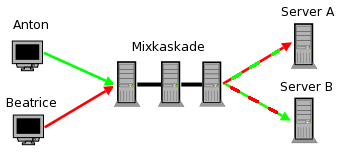
\includegraphics[scale=0.55]{../grafiken/jap.png}
\caption{Prinzip von JonDonym}
\label{abb:jap_prinzip}
\end{center}
\end{figure}

Der Dienst bietet derzeit kostenfrei nutzbare Mix-Kaskaden und Premium-Kaskaden, die nur gegen Bezahlung nutzbar sind. Die kostenfreien Mix-Kaskaden bieten nur eine geringe Geschwindigkeit von 30-50 kB/s und sind nur f�r anonymes Surfen nutzbar. Erst mit den Premium-Kaskaden entfaltet der Dienst seine volle Leistung. Diese Kaskaden bieten hohe Geschwindigkeit und sind f�r alle Protokolle nutzbar (Instant-Messaging, SSH, E-Mail\dots).\\

Anonymes Surfen erfordert mehr, als nur die IP-Adresse zu verstecken. Der JonDoFox ist ein Profil f�r Firefox, dass optimal f�r diese Aufgabe vorbereitet ist (auch f�r Tor geeignet).\\

Strafverfolgung: Einzelne Verbindungen k�nnen bei JonDonym gezielt �berwacht werden, wenn alle Betreiber einer Mix-Kaskade einen richterlichen Beschluss in ihrem Land erhalten. F�r Mix-Betreiber aus Deutschland ist eine Gerichtsbeschluss nach �100a StPO n�tig. Im Gegensatz zu Tor und I2P ist damit eine Verfolgung schwerer Verbrechen prinzipiell m�glich.\\

Die internationale Verteilung der Kaskaden verhindert eine pauschale �berwachung. Inzwischen sind alle kostenfreien und Premium-Kaskaden internationalisiert. Nach Aussage von JonDos gab es bisher noch nie eine internationale Zusammenarbeit der Beh�rden bei einer �ber�wachung und damit auch keine �berwachung der Premium-Kaskaden. Politische Aktivisten k�nnen das Risiko weiter minimieren, indem sie Kaskaden ohne deutsche Mixe nutzen.\\

Schn�ffelnde Mix-Server wurden bisher nicht bekannt.

\subsection{Testergebnisse von Computer-Zeitschriften} 
Popul�r unter den Surfern ist vor allem Tor Onion Router. Die Testergebnisse von verschiedenen Zeitschriften empfehlen jedoch meist JonDonym, da die Software JonDo+JonDoFox besser gegen Deanonymisierung durch Browserspuren sch�tzt. I2P, Freenet und RetroShare werden meist nicht in die Auswahl der getesteten Dienste einbezogen.\\

\begin{itemize}
 \item Test der Anonymisierungs�dienste in Chip Nov. 2009
 \begin{quote}
  \textit{Wer so anonym wie m�glich surfen m�chte, sollte zum Premium-Paket von JonDo greifen und das optionale JonDoFox ins�tallieren. Kein anderer Client bietet dem User einen so transparenten Service und vielf�ltige Einstellungen.}
 \end{quote} 
 \item Test der Anonymisierungs�dienste c't 18/2011
\begin{quote}
 \textit{Es gibt mehrere Pakete wie Xerobank oder das TOR Browser Bundle [...] Doch alle uns bekannten setzen auf einen veralteten Browser, kosten viel zu viel oder lassen L�cken. Bei JonDonym bekommt man dagegen zusammen mit dem Firefox-Profil JonDoFox ein besonders einfach einzurichtendes und zu nutzendes System in deutscher Sprache [...] Es ist auch das einzige Paket, das sich wirksam um die Pers�nlichkeitsspuren im Browser k�mmert.}
\end{quote}
\end{itemize}

Lediglich die ComputerBild kommt bei ihren j�hrlichen Tests zu anderen Ergebnissen und setzt regelm��ig den VPN-Anbieter CyberGhost auf den ersten Platz. M�glicherweise ist CyberGhost ein guter Anzeigenkunde?\\

Die c't schreibt in ihrem Test im Heft 18/2011 �ber VPNs:
 \begin{quote}
\textit{Bei VPNs und Proxies liegt die Information [...] beim Betreiber komplett vor, sodass eine gerichtliche Anfrage oder ein Hacker-Einbruch gen�gt, um die Anonymit�t komplett aufzuheben. Dagegen wei� bei einer Proxy-Kaskade kein Beteiligter alles �ber Herkunft und Ziel der Daten Proxy-Kaskaden verbergen also die IP-Adresse am wirksamsten...}
\end{quote} 
Also lasst die Finger davon.

\subsection{Finanzierung der Anonymisierungsdienste}
Wie wird die Entwicklung der Software und die Infrastruktur des Dienstes finanziert und welche Abh�ngigkeiten ergeben sich m�glicherweise daraus?

\subsubsection*{Tor Onion Router}
Die Softwareentwicklung wird durch Spenden finanziert. TorProject.org ben�tigt pro Jahr ca. 1 Mio. Dollar f�r die Weiterentwicklung der Software und den Betrieb weniger Kernkomponenten des Dienstes. Die Grafik \ref{abb:tor_funding} zeigt die Zusammensetzung der Spender f�r 2009 (Quelle Tor Financial Report 2009).\\

\begin{figure}[htb]
\begin{center}
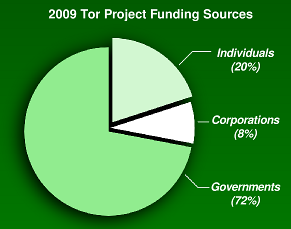
\includegraphics[scale=0.60]{../grafiken/tor-2009-funding-chart.png}
\caption{Anteil der Finanzierung von TorProject.org}
\label{abb:tor_funding}
\end{center}
\end{figure}

Die Hauptsponsoren der NGOs, Companies und Einzelspender werden von TorProject.org auf der Webseite \href{https://www.torproject.org/about/sponsors.html.en}{https://www.torproject.org/about/sponsors.html.en} ver�ffentlicht. Der gro�e Anteil ``Gouvernments'' (72\% der Einnahmen) kommt von US-Regierungsorganisationen und zu einem kleineren Teil von der schwedischen Regierung. Diese Spenden werden nicht einzeln aufgelistet. \\

Der Hauptteil der Infrastruktur wird von Enthusiasten finanziert und technisch in der Freizeit betreut. Die Kosten von 600-800 Euro pro Power-Server und Jahr sind als weitere Spenden anzusehen, die in der Grafik nicht erfasst sind. Die Administratoren ziehen keinen Vorteil aus ihrem Engagement, abgesehen von einem Zwiebel-T-Shirt.

\subsubsection*{Jondonym}
In den Jahren 2000-2004 erhielt das Projekt AN.ON als Vorl�ufer von JonDonym ca. 1 Mio. Euro aus dem deutschen Forschungsetat f�r den Aufbau des Dienstes. Seit dem Ende der F�rderung bem�ht sich die JonDos GmbH, die Finanzierung durch kostenpflichtige Premium-Angebote zu sichern. F�r dieser Angebote ist eine volumenabh�ngige Geb�hr im Voraus zu bezahlen. Die Einnahmen sollen die Kosten f�r die Weiterentwicklung der Software, die Betreuung des Projektes und die Infrastruktur der Premium-Dienste decken. Diese Ziel ist noch nicht vollst�ndig erreicht. \\

Die Entwicklung der Software wird zu 70\% aus den Einnahmen der Premium-Dienste finanziert und zu 30\% aus Forschungsprojekten in Kooperation mit Universit�ten. Die Premium-Mix-Kaskaden werden kostendeckend durch Einnahmen finanziert.\\

\subsection{Security Notes}
Die Sicherheit von IP-Anonymisierern wie Tor und JonDonym ergibt sich nicht alleine aus der Qualit�t der Anonymisierungssoftware. Durch Fehler in der verwendeten Anwendung oder falsche Konfiguration kann die Anonymit�t komplett ausgehebelt werden.
\begin{itemize}
 \item Wer die Browser Google Chrome, iCap. Safari oder einen anderen auf WebKit basierenden Browser f�r anonymes Surfen verwendet, kann durch FTP-Links deanonymisiert werden. Der Anonymit�tstest von JonDonym demonstriert es. 
 \item Wer in seinem Standardbrowser nur die Proxy-Einstellungen anpasst um Tor oder JonDo zu verwenden, ist auch nicht sicher anonym. Eine Deanonymisierung ist mit WebRTC sowie Flash- oder Java-Applets m�glich. Diese Features sind unbedingt zu deaktivieren!
 \item Viele Jabber Clients (XMPP) anonymisieren DNS-Requests nicht. Der IM-Client Pidgin (Version < 2.8) hat au�erdem Probleme mit Voice- und Video-Chats. Die Proxy-Einstellungen werden bei Voice- und Video-Chats �bergangen und es ist m�glich, einen User mit einer Einladung zum Voice-Chat zu deanonymisieren.
 \item Einige Protolle �bertragen die IP-Adresse des eigenen Rechners zus�tzlich in Headern des Protokoll-Stacks. Ein Beispiel daf�r sind nicht-anonyme Peer-2-Peer Protokolle wie BitTorrent. Damit ist es ebenfalls m�glich, User zu deanonymisieren. Eine wissenschaftliche Arbeit zeigt, wie 10.000 BitTorrent Nutzer via Tor deanomisiert werden konnten.
 \item Durch Software aus fragw�rdigen Quellen k�nnen Backdoors zur Deanonymisierung ge�ffnet werden. Eine Gruppe von ANONYMOUS demonstrierte es, indem sie eine modifizierte Version des Firefox Add-on TorButton zum Download anboten, dass wirklich von einigen Tor-Nutzern verwendet wurde. Dieses Add-on enthielt eine Backdoor, um die Nutzer von einigen Tor Hidden Services mit kinderpronografischem Material zu identifizieren. Die Liste der damit deanonymisierten Surfer wurde im Herbst 2011 im Internet ver�ffentlicht.
\end{itemize}

Schlussfolgerungen:
\begin{itemize}
 \item TorProject und JonDos empfehlen f�r anonymes Surfen ausdr�cklich eine angepasste Version des Browser Mozilla Firefox (TorBrowser bzw. JonDoFox). Nur diese Konfiguration kann als wirklich sicher nach dem aktuellen Stand der Technik gelten. Die vielen Sicherheitseinstellungen dieser beiden Browser-Erweiterungen kann man nur unvollst�ndig selbst umsetzen.
 \item F�r alle weiteren Anwendungen sind die Anleitungen der Projekte zu lesen und zu respektieren. Nur die von den Entwicklern als sicher deklarierten Anwendungen sollten mit Tor oder JonDonym genutzt werden.
 \item Verwenden Sie ausschie�lich die Originalsoftware der Entwickler.
\end{itemize}

\input{surfen_jap}
\subsection{Tor f�r Debian und Ubuntu}
Einige Linux-Distributionen enthalten Tor, Vidalia und TorButton. Die Komponenten k�nnen mit dem Paketmanger der Distribution installiert werden. F�r Debian und Ubuntu sp�lt aptitude alles n�tige auf die Platte:
\begin{verbatim}
  # aptitude install tor vidalia xul-ext-torbutton
\end{verbatim}

In der Men�gruppe Internet findet man nach der Installation \textit{Vidalia (Tor GUI)}. �ber dieses Interface kann Tor bei Bedarf gestartet und gestoppt werden.

\include{surfen_zusamenfassung}

\end{document}